\documentclass[fleqn]{article}
\usepackage[utf8]{inputenc}
\usepackage[letterpaper,margin=1in]{geometry}
\usepackage{graphicx}
\usepackage[per-mode=symbol]{siunitx}
\usepackage{amsmath}
\usepackage{float}
\usepackage{listings}
\usepackage{appendix}
\usepackage{multirow}
\usepackage{makecell}
\usepackage{titling}
\DeclareSIUnit{\quad}{Quads}
\DeclareSIUnit{\Wh}{Wh}
\DeclareSIUnit{\year}{yr}
\DeclareSIUnit{\person}{person}

\pretitle{\begin{center}\large}
\posttitle{\end{center}}
\preauthor{\begin{center}\normalsize}
\postauthor{\end{center}}
\predate{\begin{center}\footnotesize}
\postdate{\end{center}}
\setlength{\droptitle}{-40pt}

\title{Homework 2\\ENERGY 293}
\author{Gabriel Buchsbaum}

\begin{document}
\lstset{language=Matlab}

\maketitle

\begin{enumerate}
\item \quad \quad \quad $I = I_L - I_0 \left(e^{\frac{qV}{kT}}-1\right)$
  \begin{equation*}
    P=IV=V\left[I_L - I_0 \left(e^{\frac{qV}{kT}}-1\right)\right]
  \end{equation*}
  \begin{equation*}
    V_{oc} = \frac{kT}{q}\ln\left(\frac{I_L}{I_0}+1\right)
  \end{equation*}
  Maximum power when $\frac{dP}{dV}=0$
  \begin{equation*}
    \frac{dP}{dV}\Bigr|_{V_m} = V_m\left(-I_0 \frac{q}{kT} e^{\frac{qV_m}{kT}} \right) + I_L - I_0 \left(e^{\frac{qV_m}{kT}}-1\right)=0
  \end{equation*}
  \begin{equation*}
    \left(-I_0 V_m \frac{q}{kT} - I_0\right)e^{\frac{qV_m}{kT}} + I_L + I_0 = 0
  \end{equation*}
  \begin{equation*}
    -\left(V_m \frac{q}{kT} + 1\right)e^{\frac{qV_m}{kT}} + \frac{I_L}{I_0} + 1 = 0
  \end{equation*}
  \begin{equation*}
    \left(V_m \frac{q}{kT} + 1\right)e^{\frac{qV_m}{kT}} = \frac{I_L}{I_0} + 1
  \end{equation*}
  \begin{equation*}
    \ln \left(\frac{qV_m}{kT} + 1\right) + \frac{qV_m}{kT} = \ln\left(\frac{I_L}{I_0}+1\right)
  \end{equation*}
  \begin{equation*}
    \frac{kT}{q}\ln \left(\frac{qV_m}{kT} + 1\right) + V_m = V_{oc}
  \end{equation*}
  This cannot be solved into elementary functions, but math software can easily find a numerical value for $V_m$.  Once this has been calculated, it is easy enough to find the value of $I_m$:
  \begin{equation*}
    I_m = I_L - I_0 \left(e^{\frac{qV_m}{kT}}-1\right)
  \end{equation*}
  From these results, it is apparent that there is a complicated relationship between $V_m$ and $V_{oc}$, but $V_m$ increases as $V_{oc}$ increases. It is not possible to find the value of $I_m$ without knowing the value of $I_0$.

\item \quad \quad \quad $V_D = V + I R_S $
  \begin{equation*}
    I_L = I + I_D
  \end{equation*}
  \begin{equation*}
    I = I_L - I_D = I_L - I_0 \left(e^{\frac{qV_D}{kT}}-1\right) = I_L - I_0 \left(e^{\frac{q\left(V + I R_S\right)}{kT}}-1\right)
  \end{equation*}
  \begin{equation*}
    e^{\frac{q\left(V + I R_S\right)}{kT}} = \frac{I_L - I}{I_0} + 1
  \end{equation*}
  \begin{equation*}
    V + I R_S = \frac{kT}{q}\ln \left(\frac{I_L - I}{I_0} + 1\right)
  \end{equation*}
  \begin{equation*}
    R_S = \frac{\frac{kT}{q}\ln \left(\frac{I_L - I}{I_0} + 1\right) - V}{I}
  \end{equation*}
  \begin{equation*}
    R_S = \frac{\frac{kT}{q}\ln \left(\frac{I_L - I_{sc}}{I_0} + 1\right)}{I_{sc}}
  \end{equation*}

\item
  I-V plots for ideal solar cells at constant irradiance, varying temperature:
  \begin{center}
    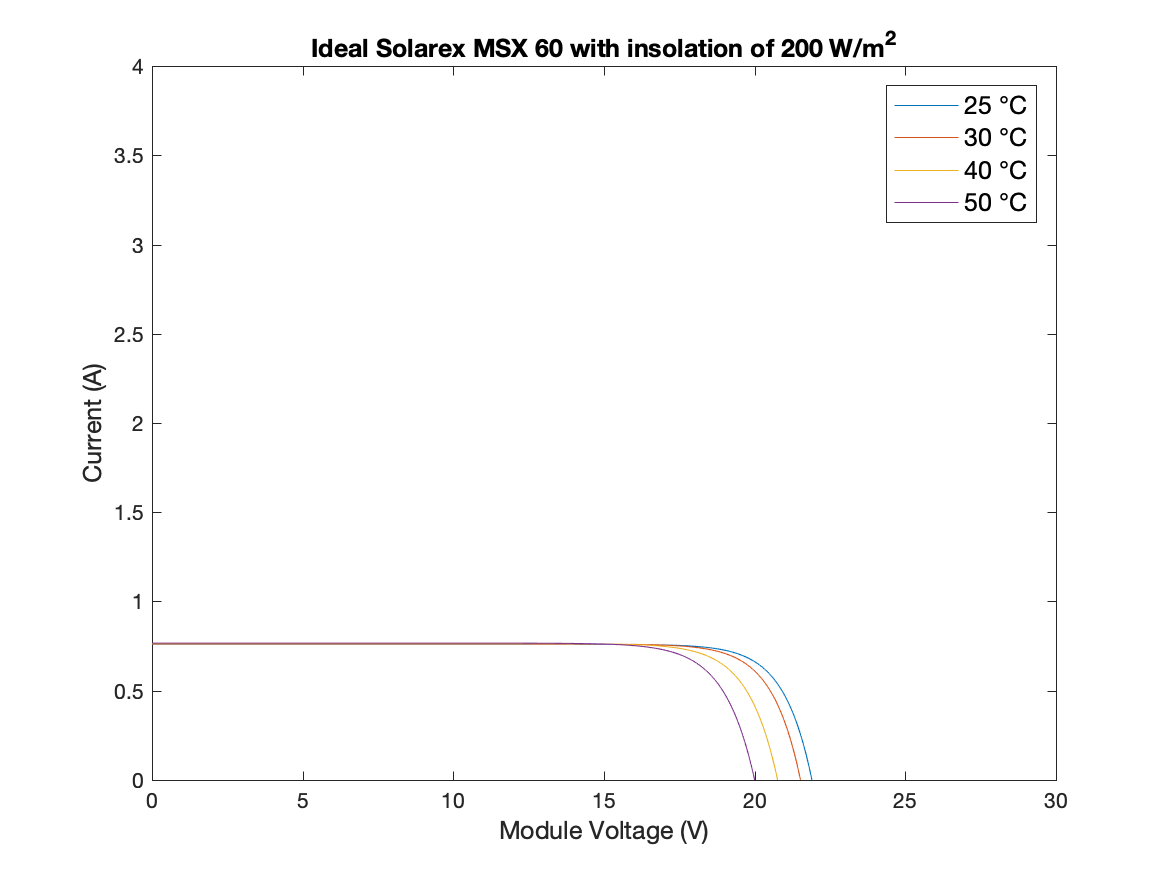
\includegraphics[width=0.9\linewidth]{200W-i.png}
  \end{center}
  \begin{center}
    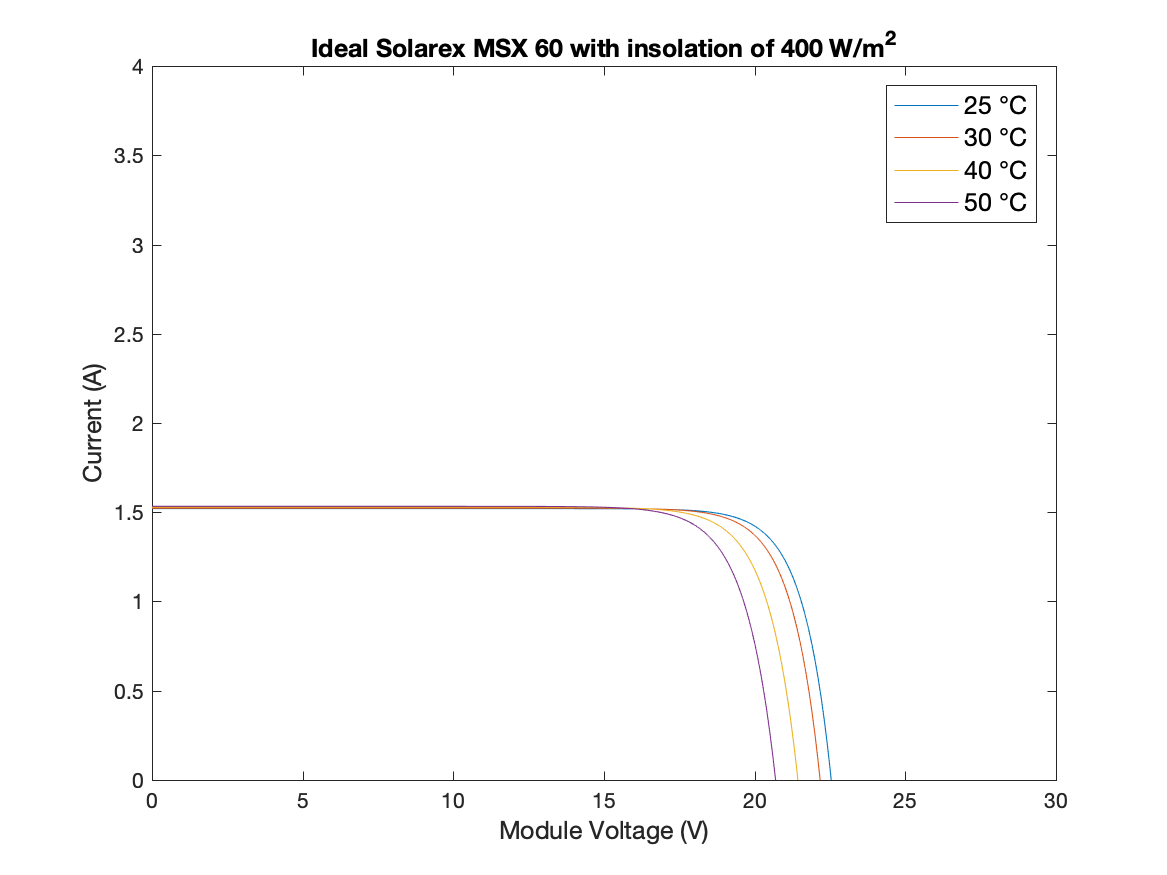
\includegraphics[width=0.9\linewidth]{400W-i.png}
  \end{center}
  \begin{center}
    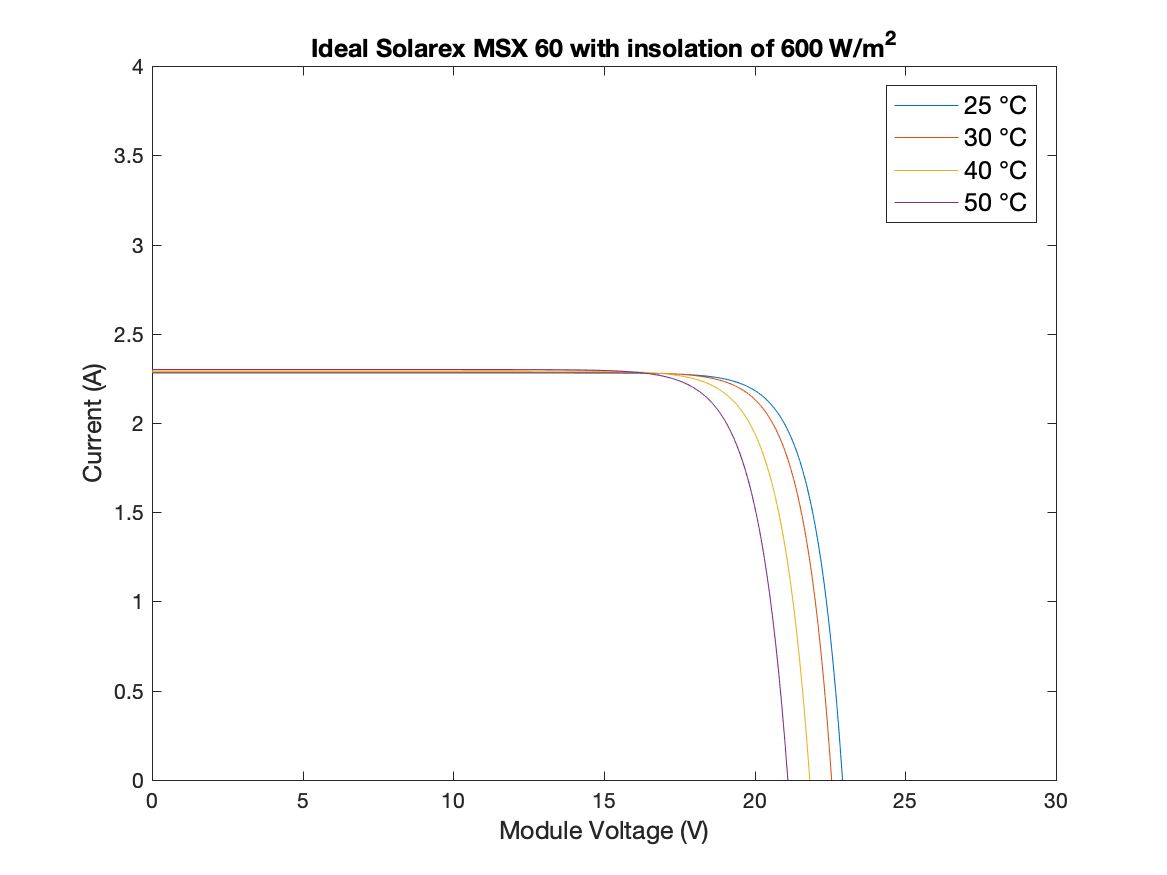
\includegraphics[width=0.9\linewidth]{600W-i.png}
  \end{center}
  \begin{center}
    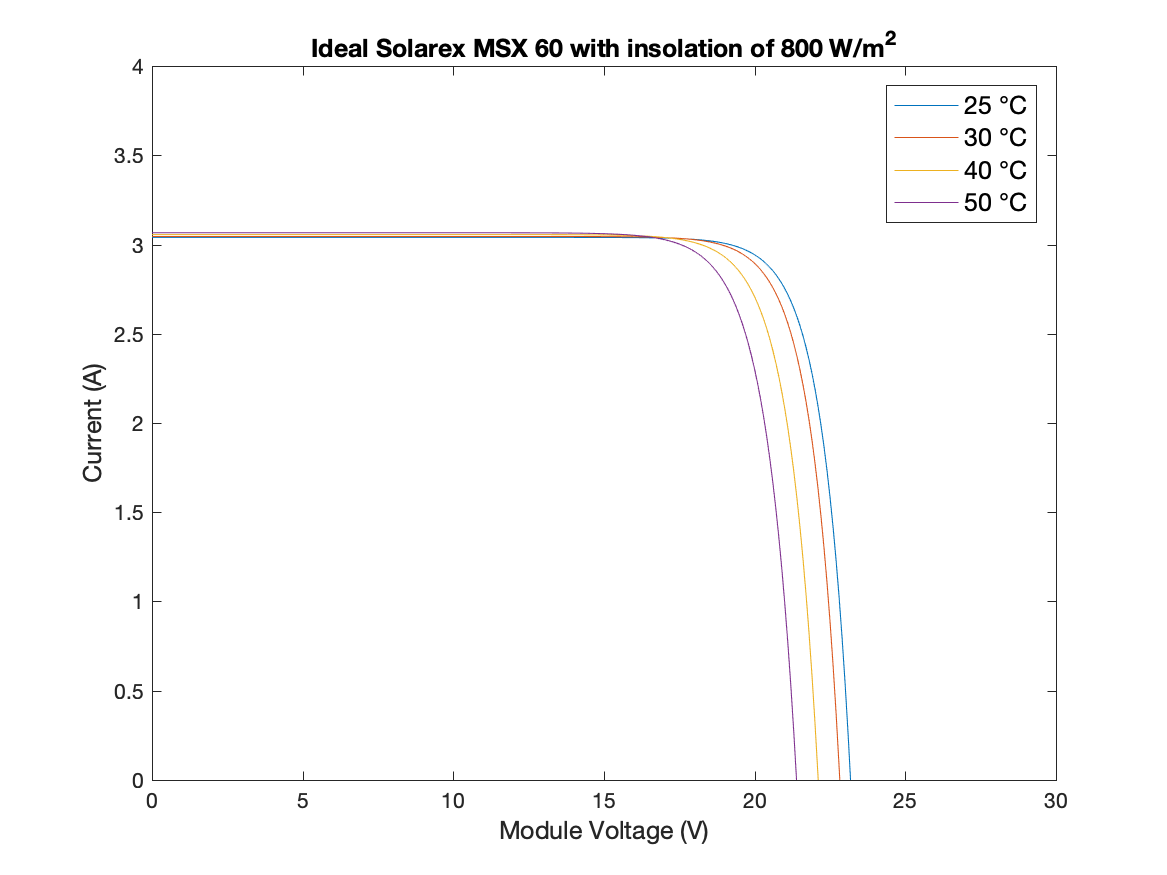
\includegraphics[width=0.9\linewidth]{800W-i.png}
  \end{center}
  \begin{center}
    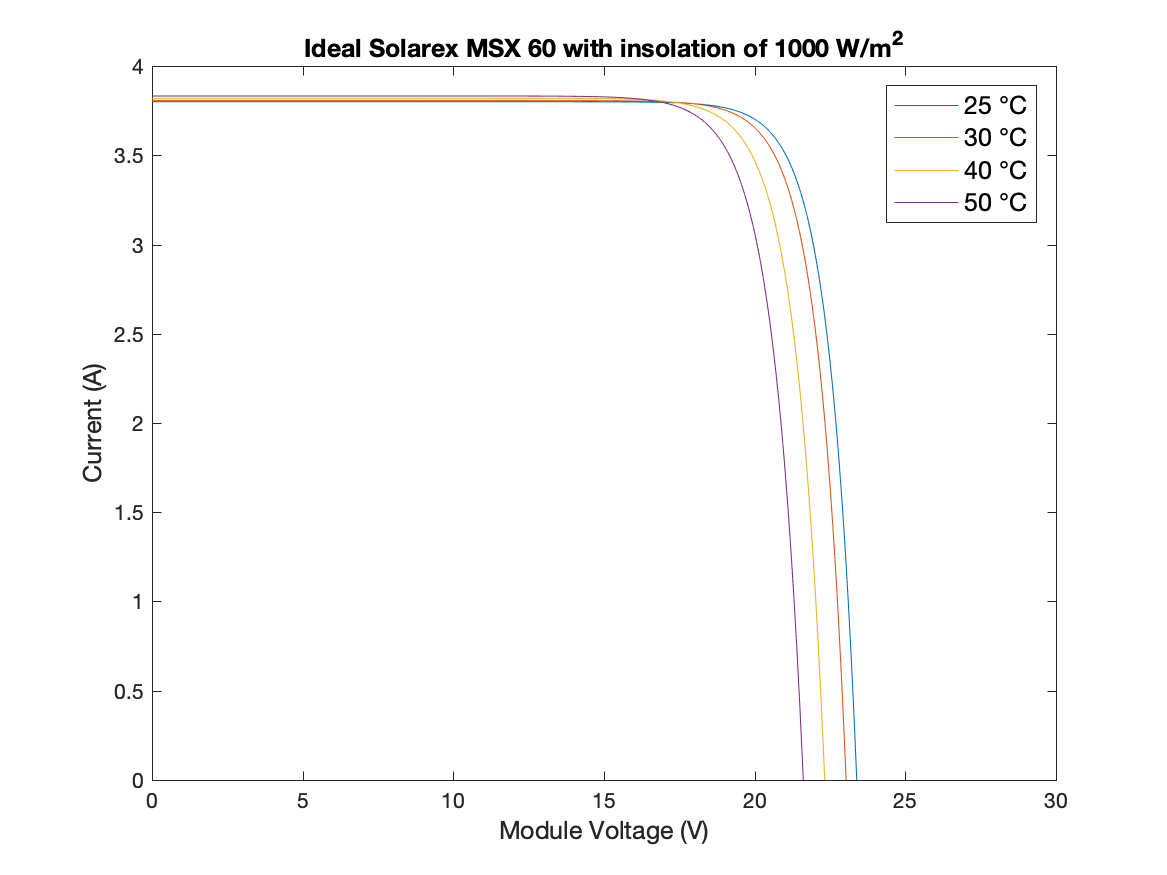
\includegraphics[width=0.9\linewidth]{1000W-i.png}
  \end{center}

  I-V plots for ideal solar cells at constant temperature, varying irradiance:
  \begin{center}
    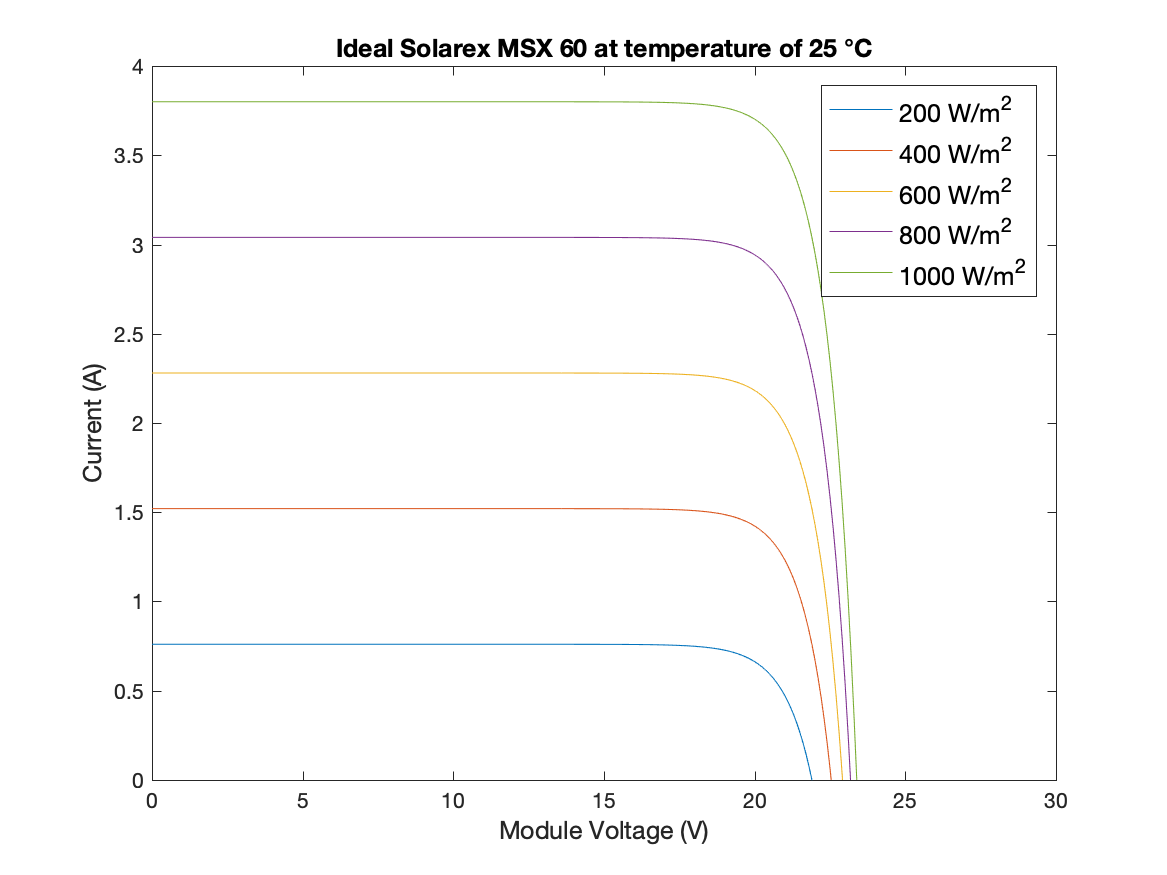
\includegraphics[width=0.9\linewidth]{25C-i.png}
  \end{center}
  \begin{center}
    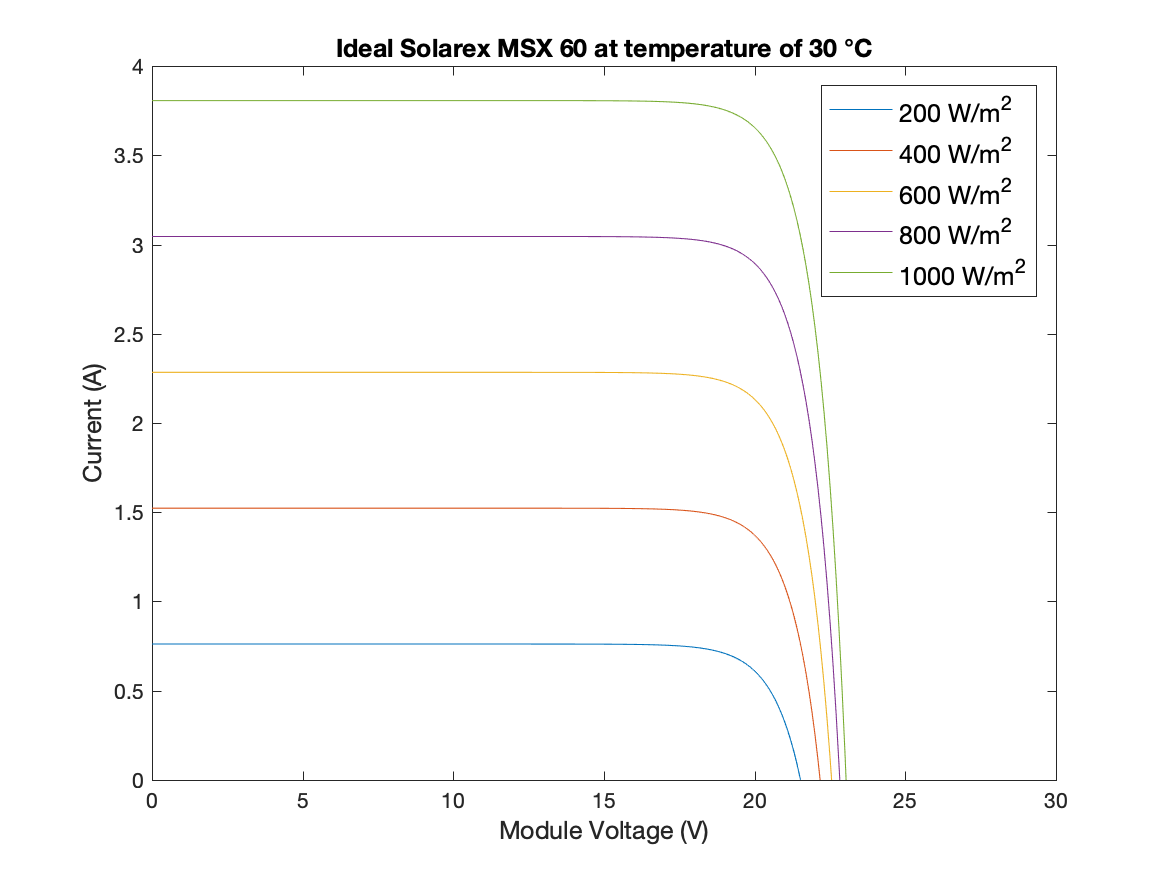
\includegraphics[width=0.9\linewidth]{30C-i.png}
  \end{center}
  \begin{center}
    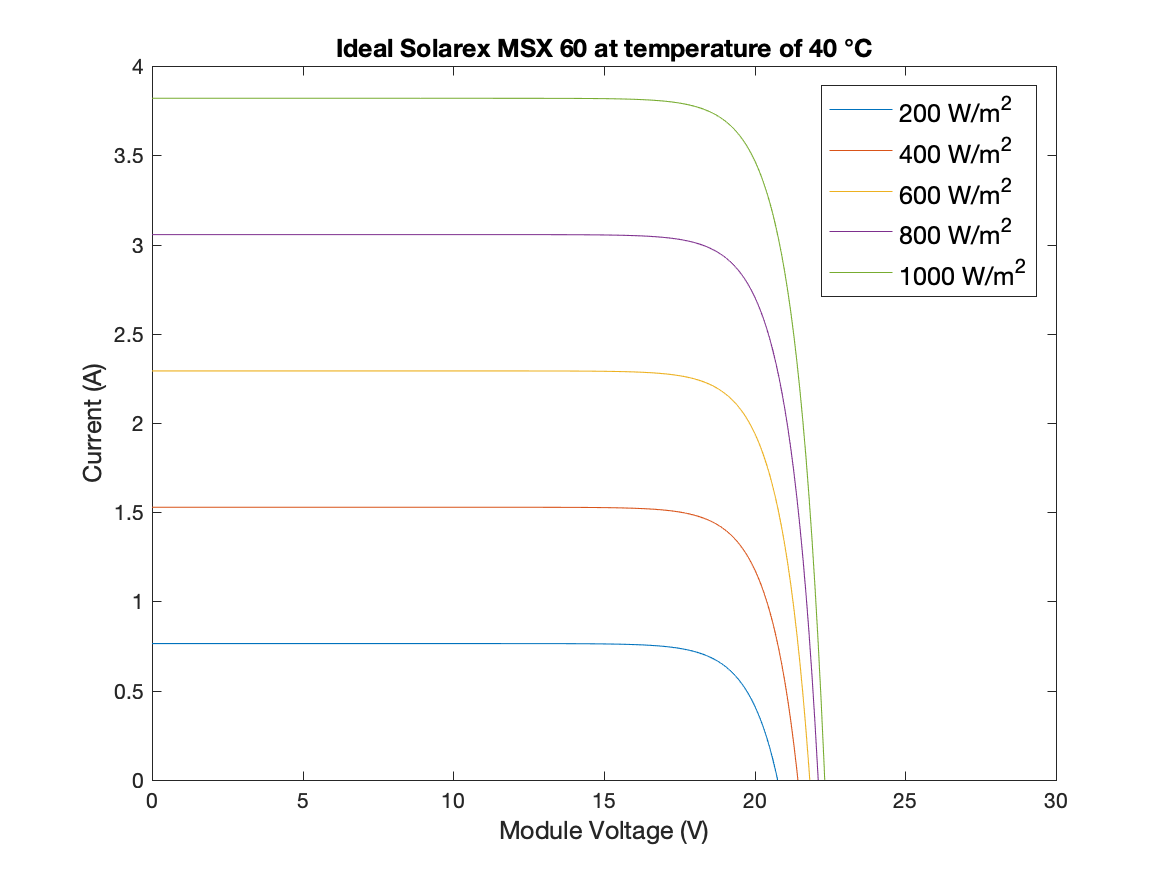
\includegraphics[width=0.9\linewidth]{40C-i.png}
  \end{center}
  \begin{center}
    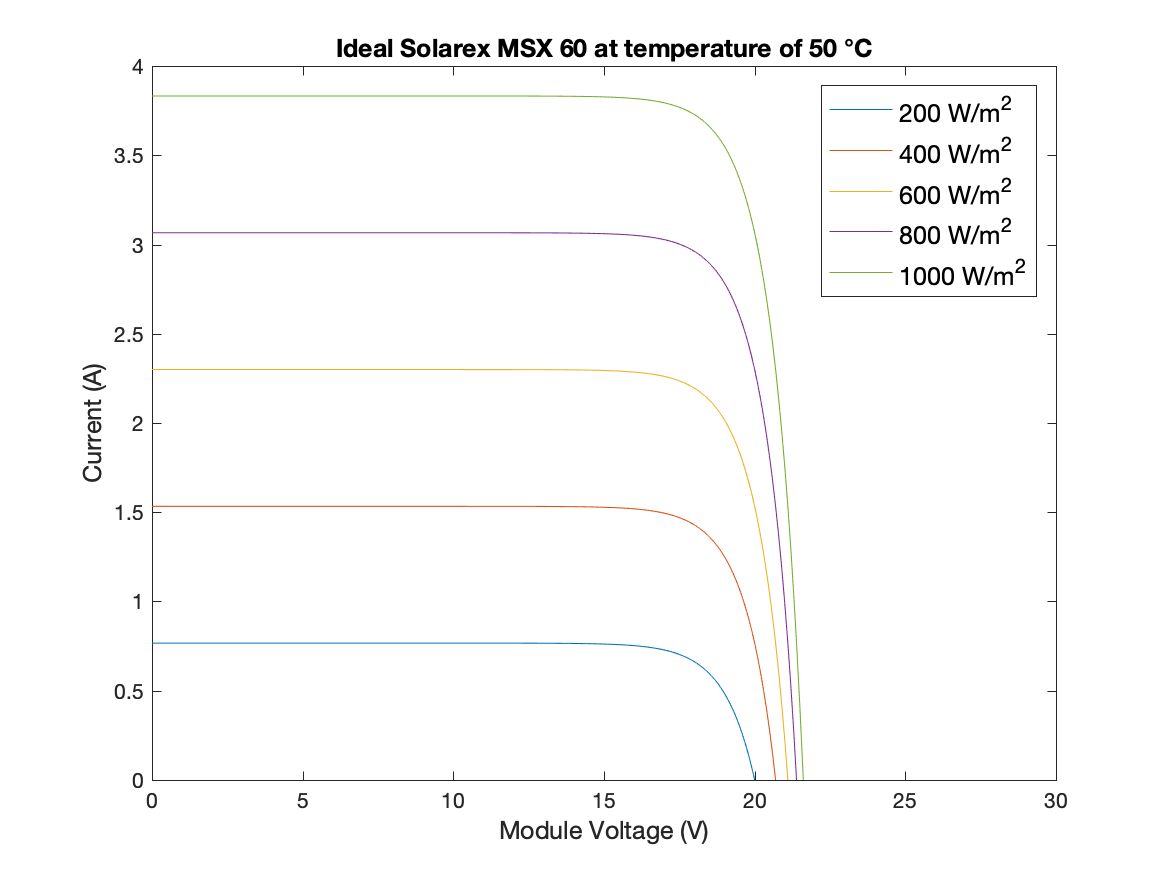
\includegraphics[width=0.9\linewidth]{50C-i.png}
  \end{center}
  
  I-V plots for solar cells with $R_s$ and $R_{sh}$ at constant irradiance, varying temperature:
  \begin{center}
    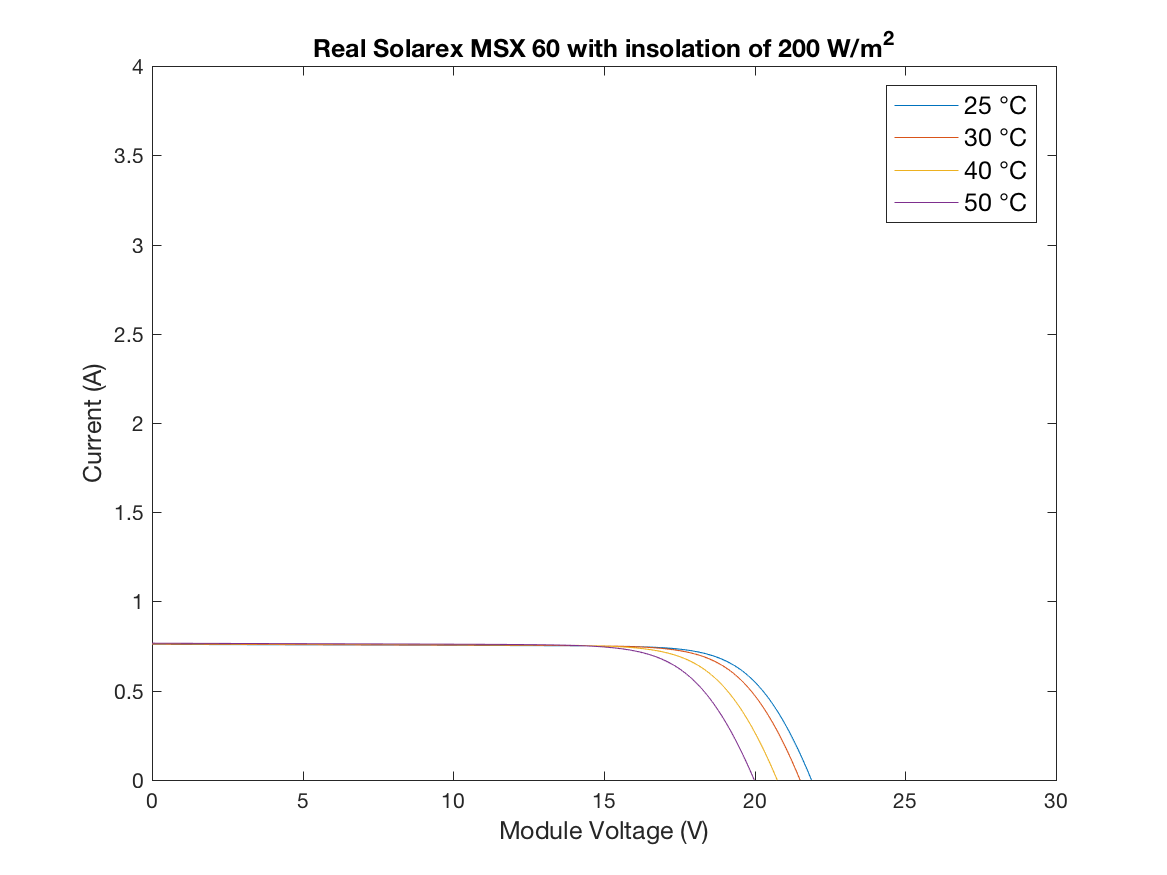
\includegraphics[width=0.9\linewidth]{200W-r.png}
  \end{center}
  \begin{center}
    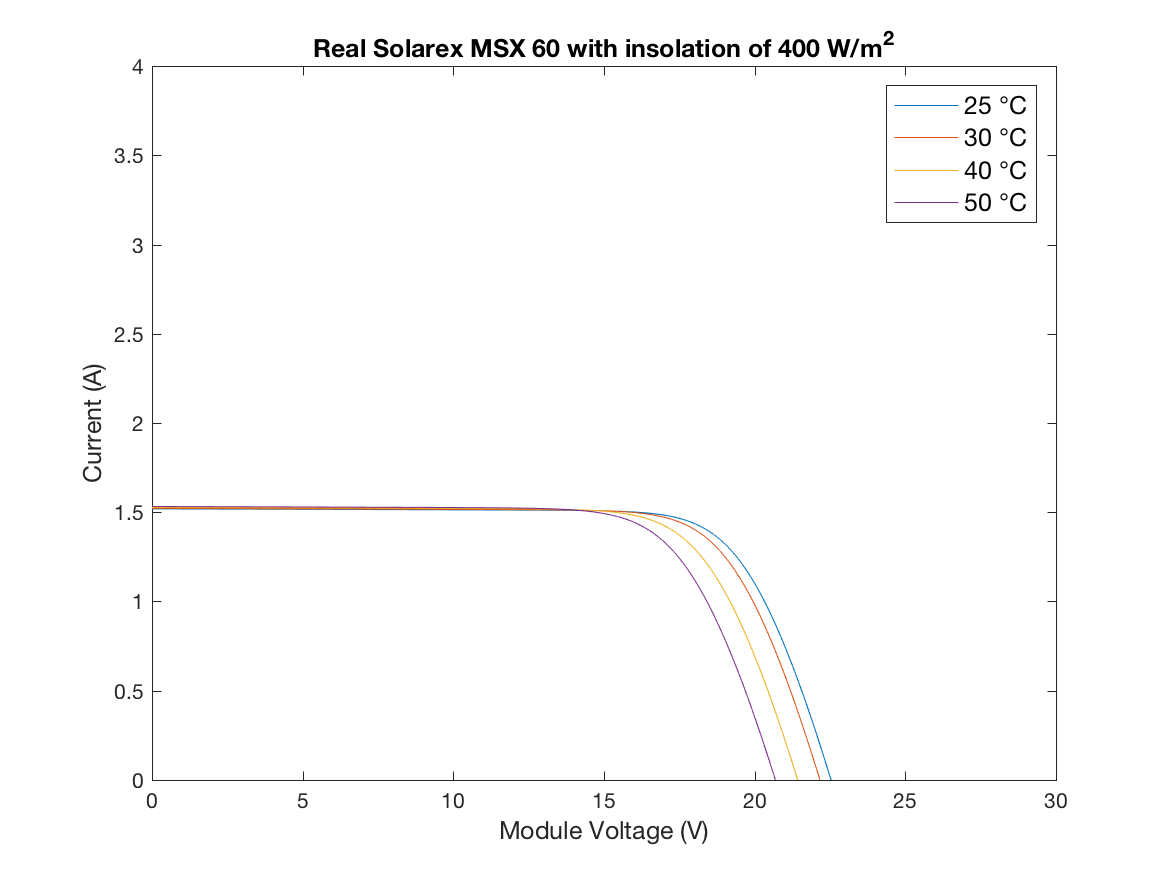
\includegraphics[width=0.9\linewidth]{400W-r.png}
  \end{center}
  \begin{center}
    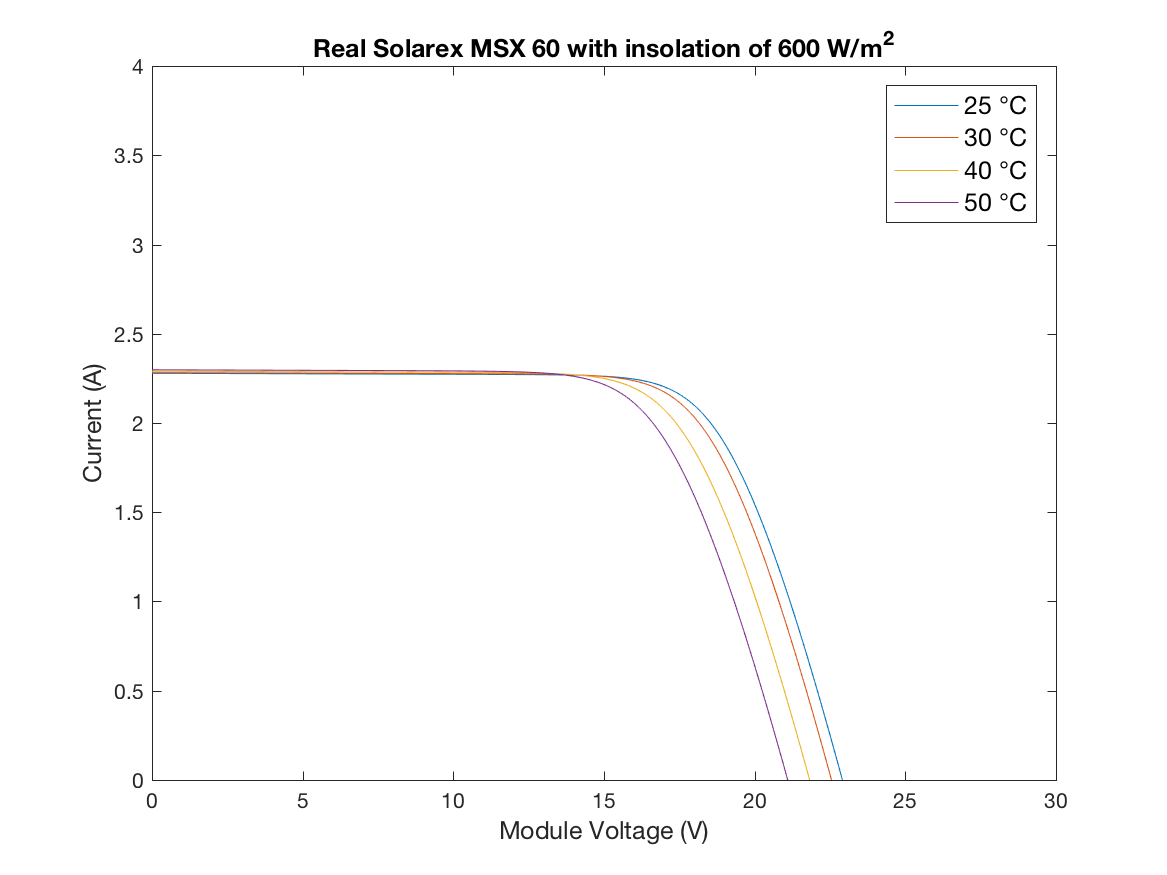
\includegraphics[width=0.9\linewidth]{600W-r.png}
  \end{center}
  \begin{center}
    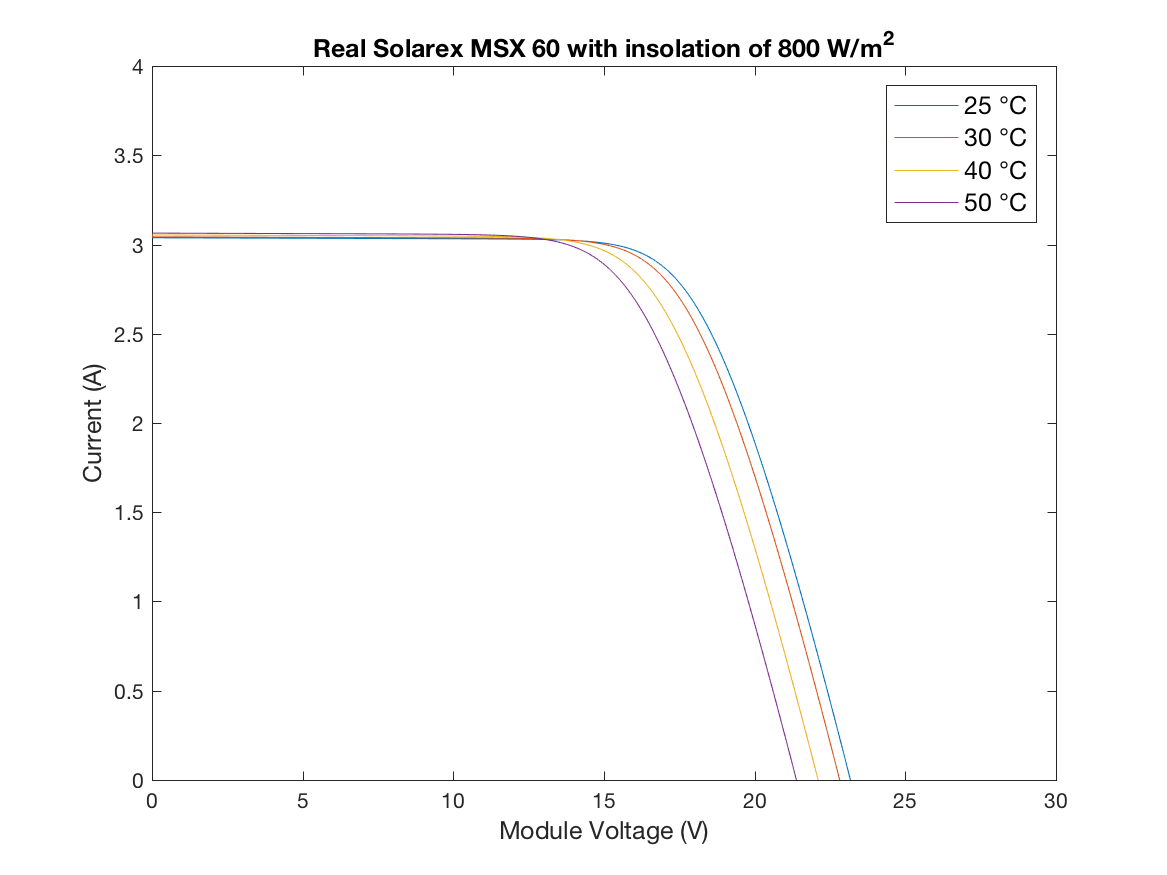
\includegraphics[width=0.9\linewidth]{800W-r.png}
  \end{center}
  \begin{center}
    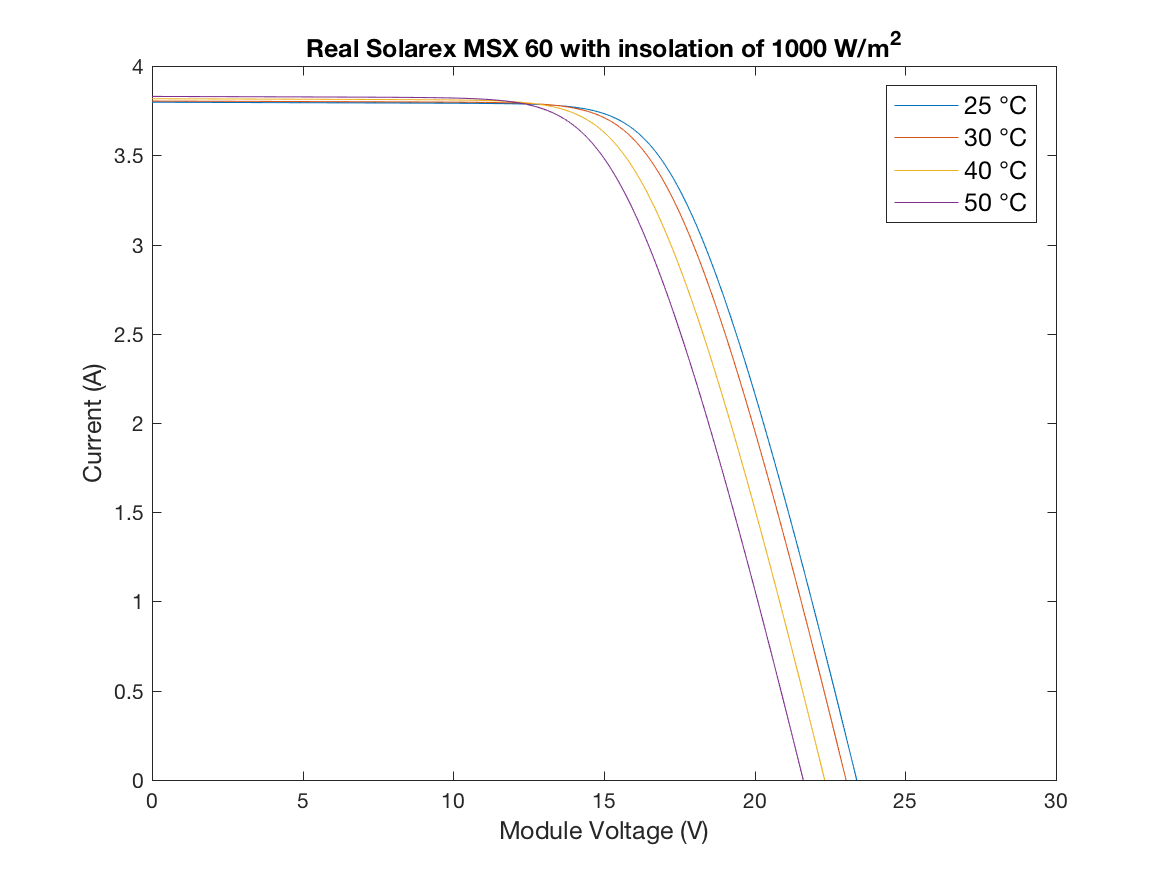
\includegraphics[width=0.9\linewidth]{1000W-r.png}
  \end{center}
  
  \pagebreak
  I-V plots for solar cells with $R_s$ and $R_{sh}$ at constant temperature, varying irradiance:
  \begin{center}
    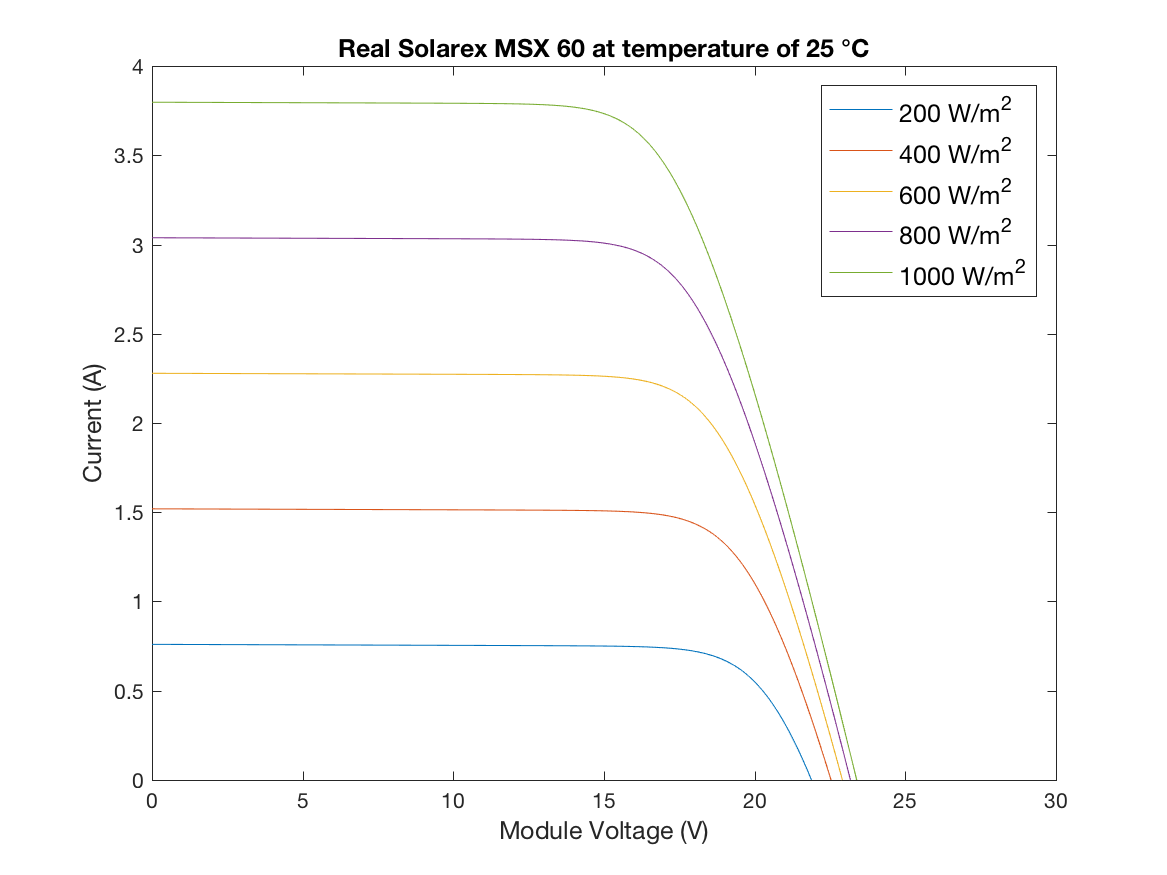
\includegraphics[width=0.9\linewidth]{25C-r.png}
  \end{center}
  \begin{center}
    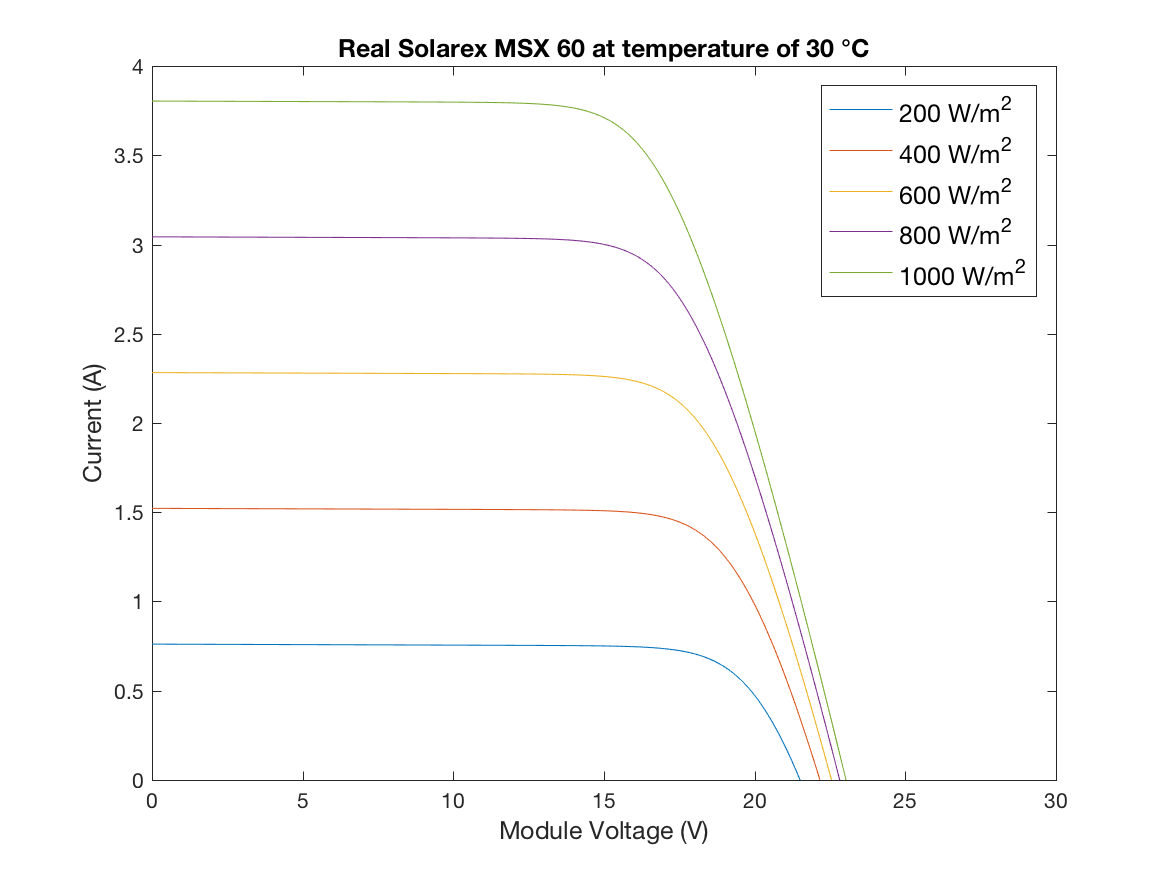
\includegraphics[width=0.9\linewidth]{30C-r.png}
  \end{center}
  \begin{center}
    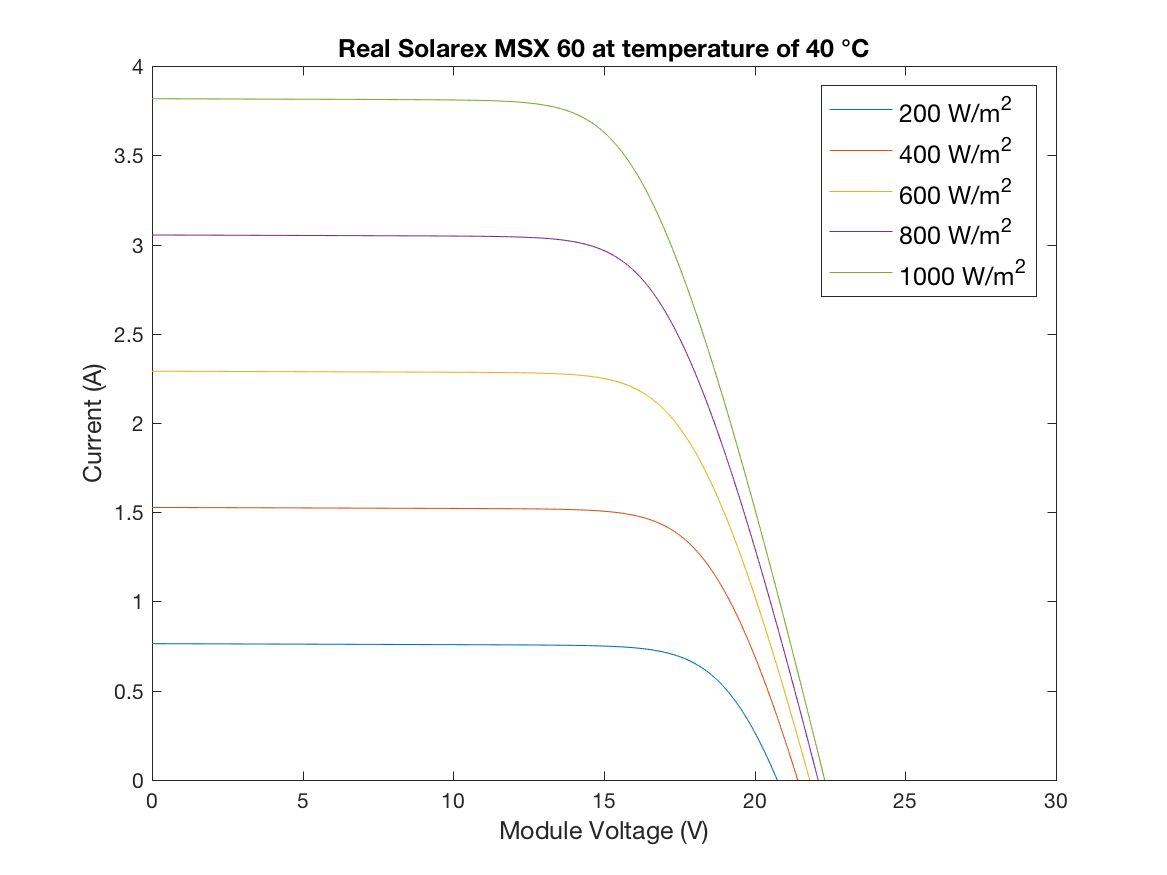
\includegraphics[width=0.9\linewidth]{40C-r.png}
  \end{center}
  \begin{center}
    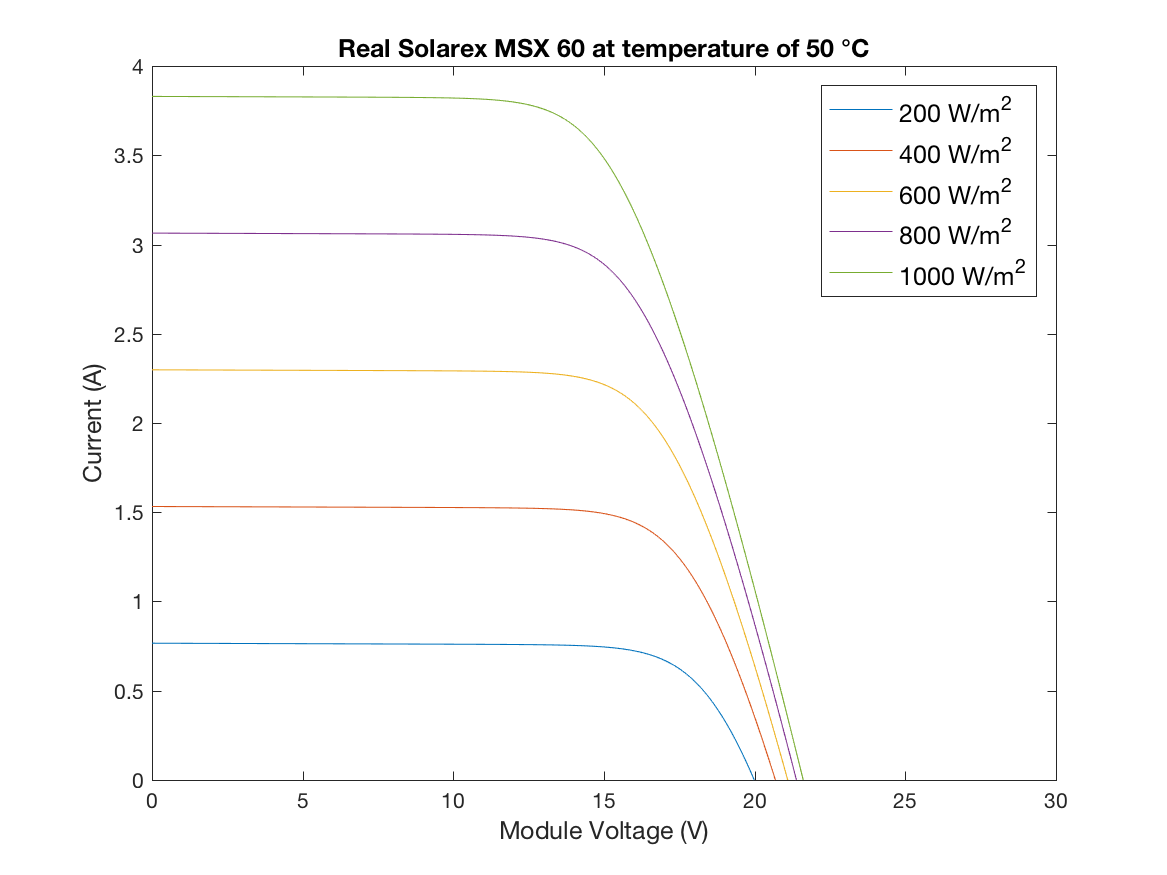
\includegraphics[width=0.9\linewidth]{50C-r.png}
  \end{center}

  \pagebreak
  Max power (in Watts) of an ideal solar module under each set of conditions:

  \begin{tabular}{|c|c|c|c|c|c|c|}
    \cline{3-7}
    \multicolumn{2}{c|}{\multirow{2}{*}{}} & \multicolumn{5}{c|}{Irradiance (\SI{}{\watt\per\meter\squared})} \\
    \cline{3-7}
    \multicolumn{2}{c|}{} & 200 & 400 & 600 & 800 & 1000 \\
    \hline
    \multirow{4}{*}{\makecell{Temperature \\ (\SI{}{\celsius})}}& 25 & 13.8 & 28.6 & 43.6 & 59.0 & 74.5 \\
    \cline{2-7}
    & 30 & 13.5 & 28.0 & 42.8 & 57.9 & 73.1 \\
    \cline{2-7}
    & 40 & 13.0 & 26.9 & 41.2 & 55.7 & 70.4 \\
    \cline{2-7}
    & 50 & 12.4 & 25.8 & 39.5 & 53.6 & 67.8 \\
    \hline
  \end{tabular}

  \vspace{\baselineskip}
  Max power (in Watts) of a solar module with $R_s$ and $R_{sh}$ under each set of conditions:

  \begin{tabular}{|c|c|c|c|c|c|c|}
    \cline{3-7}
    \multicolumn{2}{c|}{\multirow{2}{*}{}} & \multicolumn{5}{c|}{Irradiance (\SI{}{\watt\per\meter\squared})} \\
    \cline{3-7}
    \multicolumn{2}{c|}{} & 200 & 400 & 600 & 800 & 1000 \\
    \hline
    \multirow{4}{*}{\makecell{Temperature \\ (\SI{}{\celsius})}}& 25 & 13.0 & 25.9 & 37.9 & 48.9 & 58.8 \\
    \cline{2-7}
    & 30 & 12.7 & 25.3 & 37.0 & 47.8 & 57.5 \\
    \cline{2-7}
    & 40 & 12.2 & 24.2 & 35.4 & 45.7 & 54.9 \\
    \cline{2-7}
    & 50 & 11.6 & 23.1 & 33.8 & 43.5 & 52.3 \\
    \hline
  \end{tabular}

  \vspace{\baselineskip}
  From these results, a few observations are clear:
  \begin{itemize}
  \item Increasing temperature results in slightly increased short-circuit current, but decreased open-circuit voltage, and thus a decrease in maximum power.
  \item Increasing irradiance results in a proportional increase in short-circuit current, as well as a slight increase in open-circuit voltage, resulting in a more-than-proportional increase in maximum power.
  \item Adding in series and shunt resistances causes only negligible decreases in short-circuit current and open-circuit voltage.  However, it can significantly decrease the voltage that maximum power occurs at, resulting in a significant decrease in maximum power.  This effect is much more pronounced at higher irradiances than at lower irradiances. In fact, while $V_m$ increases with irradiance for ideal cells, it decreases with irradiance for 'real' cells.
  \end{itemize}
  Note: these results assume that the given series resistance of \SI{1.2}{\ohm} is for the whole modues, i.e. that each individual cell only has an equivalent series resistance of 1/36 that value.  If given resistance is the value for each individual cell, the following (clearly ineffective) result occurs:

  \begin{center}
    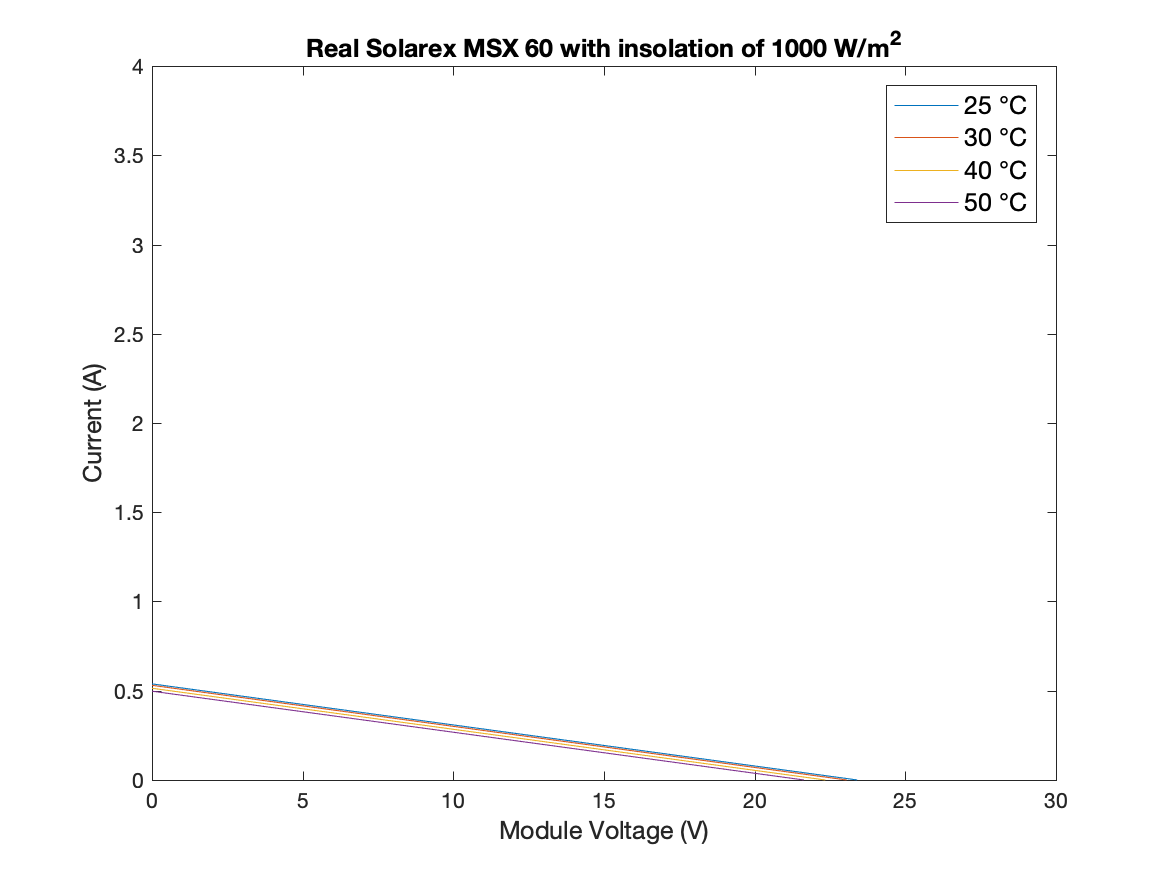
\includegraphics[width=0.75\linewidth]{1000W-r2.png}
  \end{center}
\end{enumerate}

\appendix
\setcounter{secnumdepth}{0}
\section{Appendix: Matlab code}
\begin{lstlisting}
  % close all plots and delete all existing variables to prevent conflicts
  close all
  clearvars

  % Physical constants
  q = 1.6 * 10^-19; % electron charge, C
  k = 1.38 * 10^-23; % Boltzmann constant, J/K
  Eq = 1.16; % silicon bandgap, eV

  % Specifications
  Pm = 60; % maximum power, W
  Vm = 17.1; % voltage at maximum power, V
  Im = 3.5; % current at maximum power, A
  Isc = 3.8; % short circuit current, A
  Voc = 21.1; % open circuit voltage, V
  nSeries = 36; % number of cells in series

  % Reference conditions
  musc = 1.3 * 10^-3; % change in photocurrent with temperature, A/K
  Tnom = 298; % temperature at STC, K
  Gref = 1000; % irradiance at STC, W/m^2
  I0ref = 4.0 * 10^-11; % reverse saturation current at STC, A
  ILref = Isc; % light induced current at STC, A

  % Irradiances and temperatures considered
  Grange = [200,400,600,800,1000];
  Trange = [25,30,40,50];

  % Set basic instructions
  options = optimoptions('fsolve','Display','none'); % solver options
  step = 0.1; % step size in plots
  len = ceil(24/step); % number of data points in plots (up to 24 V)
  fsize = 12; % font size in plots

  % Set up arrays to hold results
  % Results at each voltage
  Videal = zeros(20,len);
  Iideal = zeros(20,len);
  Pideal = zeros(20,len);
  % Specific module parameters
  VocIdeal = zeros(4,5);
  IscIdeal = zeros(4,5);
  PmIdeal = zeros(4,5);
  VmIdeal = zeros(4,5);
  ImIdeal = zeros(4,5);

  % Make calculations assuming ideal solar cells
  for g = 1:5
  figure
  hold on
  G = Grange(g); % choose desired irradiance
      for t = 1:4
          T = Trange(t) + 273; % choose desired temperature, and conver to K
          % Calculate I0 and IL at given irradiance and temperature
          I0 = I0ref * (T / Tnom)^3 * exp(q * Eq / k * (1 / Tnom - 1 / T));
          IL = G/Gref * (ILref + musc * (T-Tnom));
          % Calculate Vt at given temperature (for clarity and faster
          % calculations)
          Vt = k * T / q;
          
          % Calculate Voc, and determine number of points to go one point
          % past it
          eqn1 = @(V) IL - I0 * (exp(V/nSeries / Vt)-1);
          VocIdeal(t,g) = fsolve(eqn1,20,options);
          ilim = ceil(VocIdeal(t,g)/step)+1;
          
          % Cycle through each module voltage, converting to cell voltage and
          % calculating current from that. Power is calculated by multiplying
          % current and module voltage. The method used to store results
          % means that each plot must have the same number of points;
          % however, it is a waste of time to calculate data beyond the Voc.
          % As a result, P and V values beyond the first point above Voc are
          % left as zero, while I values are set to -1 to avoid showing up on
          % the plot.
          for i = 1:len
              if i <= ilim
                  Vmodule = (i-1)*step;
                  Vc = Vmodule / nSeries; % cell voltage
                  Videal(4*(g-1)+t,i) = Vmodule;
                  Iideal(4*(g-1)+t,i) = IL - I0 * (exp(Vc / Vt)-1);
                  Pideal(4*(g-1)+t,i)=Iideal(4*(g-1)+t,i)*Videal(4*(g-1)+t,i);
              else
                  Iideal(4*(g-1)+t,i) = -1;
              end
          end
          % Add results to plot
          plot(Videal(4*(g-1)+t,:),Iideal(4*(g-1)+t,:))
          % Short circuit current is current at V = 0
          IscIdeal(t,g) = Iideal(4*(g-1)+t,1);
          % Max power is found by finding highest value of power in array.
          % Since it is only calculated at every 0.1 V, it is moderately less
          % precise than solving for the maximum, but the added precision is
          % not worth the complexity, particulary for the 'real' module.
          [PmIdeal(t,g),index] = max(Pideal(4*(g-1)+t,:));
          VmIdeal(t,g) = Videal(4*(g-1)+t,index);
          ImIdeal(t,g) = Iideal(4*(g-1)+t,index);
      end
      % Set up plot. These plots show how temperature affects the IV curve at
      % a given irradiance.
      xlim([0,30]);
      ylim([0,4]);
      xlabel('Module Voltage (V)','Fontsize',fsize);
      ylabel('Current (A)','Fontsize',fsize);
      legend({'25 C','30 C','40 C','50 C'},'Fontsize',fsize)
      ttl = ['Ideal Solarex MSX 60 with insolation of ',int2str(G),' W/m^2'];
      title(ttl,'Fontsize',fsize)
      box on
      saveas(gcf,[int2str(G),'W-i.png'])
      hold off
  end
  
  % Redo plots to show how irradiance affects the IV curve at a given
  % temperature
  for t = 1:4
      figure
      hold on
      T = Trange(t);
      for g = 1:5
          plot(Videal(4*(g-1)+t,:),Iideal(4*(g-1)+t,:))
      end
      xlim([0,30]);
      ylim([0,4]);
      xlabel('Module Voltage (V)','Fontsize',fsize);
      ylabel('Current (A)','Fontsize',fsize);
      lgd = {'200 W/m^2','400 W/m^2','600 W/m^2','800 W/m^2','1000 W/m^2'};
      legend(lgd,'Fontsize',fsize)
      ttl = ['Ideal Solarex MSX 60 at temperature of ',int2str(T),' C'];
      title(ttl,'Fontsize',fsize)
      box on
      saveas(gcf,[int2str(T),'C-i.png'])
      hold off
  end
  
  % Input the given series and shunt resistance. This assumes that the given
  % series resistance applies to the whole module, and hence divides it by
  % the number of cells to determine how each individual cell behaves.
  Rs = 1.2/nSeries;
  Rsh = 50;
  
  % Again, set up arrays to store results
  Vreal = zeros(20,len);
  Ireal = zeros(20,len);
  Preal = zeros(20,len);
  VocReal = zeros(4,5);
  IscReal = zeros(4,5);
  PmReal = zeros(4,5);
  VmReal = zeros(4,5);
  ImReal = zeros(4,5);
  
  % Perform calculations assuming solar cells have series and shunt
  % resistances. This functions the same way as the ideal cells, except for a
  % different equation for current.
  for g = 1:5
      figure
      hold on
      G = Grange(g);
      for t = 1:4
          T = Trange(t) + 273;
          I0 = I0ref * (T / Tnom)^3 * exp(q * Eq / k * (1 / Tnom - 1 / T));
          IL = G/Gref * (ILref + musc * (T-Tnom));
          Vt = k * T / q;
          
          eqn2 = @(V) IL-I0*(exp((V/nSeries)/Vt)-1)-(V/nSeries)/Rsh;
          VocReal(t,g)=fsolve(eqn2,20,options);
          ilim = ceil(VocReal(t,g)/step)+1;
          
          for i = 1:len
              if i <= ilim
                  Vmodule = (i-1)*step;
                  Vc = Vmodule / nSeries;
                  Vreal(4*(g-1)+t,i) = Vmodule;
                  % Use implicit equation solving to find current at given
                  % voltage
                  eqn3 = @(I) IL-I0*(exp((Vc+I*Rs)/Vt)-1)-(Vc+I*Rs)/Rsh-I;
                  Ireal(4*(g-1)+t,i) = fsolve(eqn3,0,options);
                  Preal(4*(g-1)+t,i) = Ireal(4*(g-1)+t,i)*Vreal(4*(g-1)+t,i);
              else
                  Ireal(4*(g-1)+t,i) = -1;
              end
          end
          plot(Vreal(4*(g-1)+t,:),Ireal(4*(g-1)+t,:))
          IscReal(t,g) = Ireal(4*(g-1)+t,1);
          [PmReal(t,g),index] = max(Preal(4*(g-1)+t,:));
          VmReal(t,g) = Vreal(4*(g-1)+t,index);
          ImReal(t,g) = Ireal(4*(g-1)+t,index);
      end
      xlim([0,30]);
      ylim([0,4]);
      xlabel('Module Voltage (V)','Fontsize',fsize);
      ylabel('Current (A)','Fontsize',fsize);
      legend({'25 C','30 C','40 C','50 C'},'Fontsize',fsize)
      ttl = ['Real Solarex MSX 60 with insolation of ',int2str(G),' W/m^2'];
      title(ttl,'Fontsize',fsize)
      box on
      saveas(gcf,[int2str(G),'W-r.png'])
      hold off
  end
  
  for t = 1:4
      figure
      hold on
      T = Trange(t);
      for g = 1:5
          plot(Vreal(4*(g-1)+t,:),Ireal(4*(g-1)+t,:))
      end
      xlim([0,30]);
      ylim([0,4]);
      xlabel('Module Voltage (V)','Fontsize',fsize);
      ylabel('Current (A)','Fontsize',fsize);
      lgd = {'200 W/m^2','400 W/m^2','600 W/m^2','800 W/m^2','1000 W/m^2'};
      legend(lgd,'Fontsize',fsize)
      ttl = ['Real Solarex MSX 60 at temperature of ',int2str(T),' C'];
      title(ttl,'Fontsize',fsize)
      box on
      saveas(gcf,[int2str(T),'C-r.png'])
      hold off
  end
  
  % Print numerical results
  VocIdeal
  VocReal
  IscIdeal
  IscReal
  PmIdeal
  PmReal
  VmIdeal
  VmReal
  ImIdeal
  ImReal
  
\end{lstlisting}

\end{document}
